
\section{Introduction}
This is a classification task based on \href{https://valueeval.webis.de/}{SemEval 2023 Task 4}. Its objective is to identify human values behind arguments.  
To be more clear, given a text and some value categories, here we want to identify which category it falls in and also is it against or in favor of that category. 

\section{Dataset}
Initially there was a dataset of 5393 annotated arguments. There was 20 values which i chose only 3 of them:
\begin{itemize}
	\item Achievement
	\item Power: dominance
	\item Power: resources
\end{itemize}
After extracting the values which we want to classify, there remains 2188 arguments.

\subsection{Data Collection}
Using requests in python, I gathered needed data from the \href{https://zenodo.org/record/7879430/files}{dataset} provided.

\subsection{Data Structure}
The annotated corpus in tab-separated value format. Contains the following files for the different dataset splits:
    arguments-<split>.tsv: Each row corresponds to one argument
        Argument ID: The unique identifier for the argument
        Conclusion: Conclusion text of the argument
        Stance: Stance of the Premise towards the Conclusion; one of "in favor of", "against"
        Premise: Premise text of the argument
    labels-<split>.tsv: Each row corresponds to one argument
        Argument ID: The unique identifier for the argument
        Other: Each other column corresponds to one value category, with a 1 meaning that the argument resorts to the value category and a 0 that not

\subsection{Data Filtering}
In this state, I joined the arguments and labels by the Argument ID. I deleted all columns and rows which were related to other values.
For each of the remaining values, there is two labels: 'against' and 'in favor of' which I showed by adding 'N' or 'P' at the end of the value name.

\subsection{Data Cleaning}
For cleaning data, I removed all punctuation marks except dot. The reason for that is it makes the sentence and word tokenizing easier.

\subsection{Data Breaking}
After cleaning the data, I broke data by its sentence. You can find the label seperated files inside data/sentencebroken directory. I also
broke data by its words which you can find the label seperated files inside data/wordbroken directory.

\section{Statistics}
These are some basics statistics about the dataset.

\subsection{Row Count}
Number of rows for each label.
\begin{adjustbox}{max width=\textwidth}
\csvautotabular{../stats/row_count.tsv}
\end{adjustbox}

\subsection{Sentence Count}
Number of sentence for each label.
\begin{adjustbox}{max width=\textwidth}
    \csvautotabular{../stats/sentence_count.tsv}
\end{adjustbox}

\subsection{Word Count}
Number of words for each label.
\begin{adjustbox}{max width=\textwidth}
    \csvautotabular{../stats/word_count.tsv}
\end{adjustbox}

\subsection{Unique Word Count}
Number of unique words for each label.
\begin{adjustbox}{max width=\textwidth}
    \csvautotabular{../stats/unique_word_count.tsv}
\end{adjustbox}

\subsection{Common Unique Word Count}
Number of common unique words for each label.  
Extra explanation: I computed the common words between all labels, then count the number of unique words for each label which are present in common words.
\begin{adjustbox}{max width=\textwidth}
    \csvautotabular{../stats/common_unique_word_count.tsv}
\end{adjustbox}

\subsection{Uncommon Unique Word Count}
Number of uncommon unique words for each label.  
Extra explanation: I computed the common words between all labels, then count the number of unique words for each label which are not present in common words.
\begin{adjustbox}{max width=\textwidth}
    \csvautotabular{../stats/uncommon_unique_word_count.tsv}
\end{adjustbox}

\subsection{10 Most Frequent Uncommon Words}
10 most frequent uncommon words for each label.  
Extra explanation: I computed the common words between all labels, then count the number of unique words occurrences for each label which are not present in common words, and sort them by number of occurrences to get the 10 most frequent uncommon words.
\begin{adjustbox}{max width=\textwidth}
    \csvautotabular{../stats/most_frequent_uncommon_words.tsv}
\end{adjustbox}

\subsection{Words Histogram}
In this words histogram, you see 30 of the most frequent words in all labels.
\begin{figure}[H]
    \begin{center}
        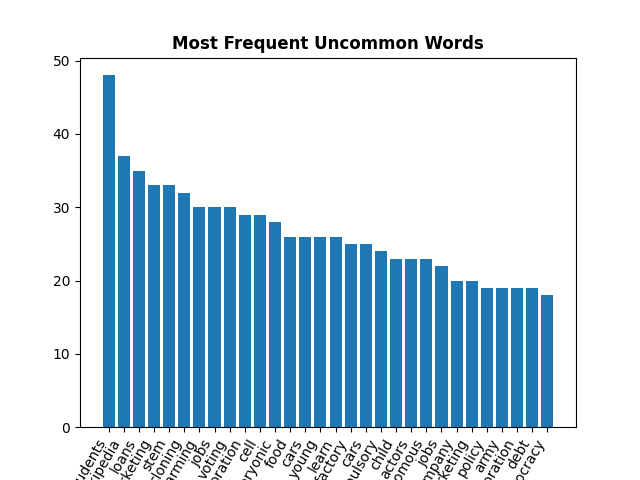
\includegraphics[width=\linewidth]{../stats/words_histogram.png}
        \caption{most Frequent Words}
    \end{center}
\end{figure}

\section{Run Script}
I wrote a python script which allows any user to run each part of this project seperately.
